\section{Introduction}

% \body{
%     Data representation plays a key role in the computational complexity of several natural problems. While some representations often increase the difficulty of the problem~\cite{GALPERIN1983183}, many efficient algorithms are designing by assuming that the input is \emph{decomposed}, or \emph{represented}, in a specific way.
%     In this paper, we introduce and explore a novel decomposition based on coordinate systems for graphs, which we call \textit{tree co-decompositions}. As we shall see, these are categorical duals of tree decompositions, and can be easily generalized to other relational structures. However, closely related constructions also appear naturally in scientific modeling, where scientists use coordinates, each corresponding to a different modeling concern, to make sense of large combinatorial objects~\cite{LibkindEtAl2022Epidemic,BaezEtAl2023StockFlowFramework}. This means that close relatives of co-decompositions can already be found ``in the wild''. This scientific modeling perspective provides us with an intuitive route towards understanding what a co-decomposition is.
% }

\body{
    Whether mathematical concepts are discovered or invented, the path by which we arrive at them is not always the best route to understanding. We came to \textit{tree co-decompositions} by dualizing a categorical generalization of tree-width~\cite{StructuredDecompositions}, where the topological viewpoint is replaced by a more algebraic one.% one organized around coordinates. 
    Yet the notion of a co-decomposition extends beyond graphs and tree-shapes: co-decompositions of vector spaces are precisely \textit{cellular sheaves}, which  play a growing role in applied topology~\cite{Curry2014,HansenGhrist2019,Robinson2017}. In this introduction, however, we choose a more natural way, at least in hindsight, and which hints at potential applications of our algorithms: the use of coordinates to organize distinct concerns in scientific modeling~\cite{LibkindEtAl2022Epidemic,BaezEtAl2023StockFlowFramework}.
}

\body{
    Suppose Letícia, an epidemiologist, is trying to understand the spread of a new disease; let's call it X. She knows that various factors influence its spread: infection dynamics, host population movement patterns, population demographics, other diseases, etc. She would prefer to model each of these aspects independently, making it is easier to reason about, communicate, and explain her findings. She sets up a disease spread model, a model to account for ageing, a model to record movement from one city to another, and a model for a separate disease, Y, which is known to interact with X. Of course, what Letícia is really after is a combined model which is appropriately stratified, in the sense that she can combine states across the various models: for instance, she might want a part corresponding to those individuals who live in São Paulo, are elderly, are exposed to X, and have recently recovered from~Y. This sort of situation arises in practice, and several mathematical frameworks have been developed for this purpose \cite{LibkindEtAl2022Epidemic,BaezEtAl2023StockFlow,BaezEtAl2023StockFlowFramework}. Some of these use \textit{fibered products}, also known as \textit{pullbacks}, to negotiate the relationships between the constituent models so that they may be assembled into a much larger model of the process Letícia actually cares about~\cite{LibkindEtAl2022Epidemic,BaezEtAl2023StockFlowFramework}. A co-decomposition is precisely such a ``recipe'' for assembling large models as fibered products of smaller pieces.
}\label{para: leticia}

\body{
    As the number of variables of the combined model increases, inference and information retrieval becomes exponentially more difficult. In practice, Letícia might cope with this intractability by describing the individual models as small combinatorial structures, which interact through what we call \emph{adhesions}. For example, she may use Petri nets to organize modelling at a high level, since the corresponding systems of differential equations can be derived automatically from the nets once the appropriate rates have been specified \cite{LibkindEtAl2022Epidemic}. Suppose abstractly that Letícia has to combine two models $G$ and $H$. She does this by first selecting an adhesion $K$, together with homomorphisms $g\colon G\to K$ and $h\colon H\to K$. She then constructs the larger model, $G\times_K H$, by taking pairs of elements of $G$ and $H$ mapped to the same point in $K$. We state this formally for graphs, but there is an analogous definition for arbitrary relational structures.
}

    \begin{definition}\label{def:pullback}
        For graphs $G,H,K$ and homomorphisms $g \colon G \to K$, $h \colon H \to K$, the \define{pullback} (or fibered product) of $G$ and $H$ along $K$ is the graph $G \times_K H$ with vertex set $V:=\{(x,y)\in V(G)\times V(H) \mid g(x)=h(y)\}$ and edge set $E:=\{((x,y),(x',y'))\in V\times V \mid (x,x')\in E(G)\wedge (y,y')\in E(H)\}$.
    \end{definition}
\body{
    The key insight here is that the relations (edges) present in $G\times_K H$ are completely determined, coordinate-wise, by the relations in $G$ and $H$, subject to the compatibility imposed by $K$. By repeating this operation for each of the smaller models she has constructed, Letícia can systematically assemble the large model she is after. If the relationships between Letícia's small models describe a tree, then the combined model is what we call a \emph{tree co-decomposition}, an example of which can be seen in the left-hand side of \cref{fig:limit}. 
}\label{para: pullback Leticia}
\newpage
\begin{definition}\label{def:tree_codecomp}
    A \define{tree co-decompsition} $\Ta$ is a triple $(T, \{G_a\},\{g_t^e\})$ such that: \vspace{-.5em}
    \begin{enumerate}
        \item $T$ is a tree;\vspace{-.5em}
        \item the family of graphs $\{G_a\}:=\{G_e\}_{e \in E(T)}\cup\{G_t\}_{t \in V(T)}$ is indexed over \textit{both} the edges $e\in E(T)$ and nodes $t\in V(T)$ of $T$; and \vspace{-.5em}
        \item each $\{g_t^e\}_{t\in V(T),e\in E(t)}$ is a family of an epimorphisms $G_t\to G_e$ indexed over the incident edges $e\in E(t)$ of each node $t\in V(T)$.\vspace{-.5em}
    \end{enumerate} 
    We call $T$ the \define{auxiliary tree}. The graphs $\{G_t\}$ indexed by nodes are the \define{bags of $\Ta$} and the graphs $\{G_e\}$ indexed by edges are the \define{adhesions of $\Ta$}; the \define{width} of $\Ta$ is its maximum bag size.
    We say that $G$ is the \define{limit} of $\Ta$ if $G$ is isomorphic to the graph obtained by recursively taking the pullbacks along the edges of $T$, i.e., $G \simeq \lim \Ta$.
    The \define{tree co-width} of $G$, denoted by $\mathsf{cow}(G)$, is the minimum among the widths of all tree co-decompositions whose limit is $G$.
    When the tree $T$ is a path, we call $\Ta$ a \define{path co-decomposition} (these admit an alternative characterization in terms of a grammar; c.f.~Appendix~\ref{appendix: grammar}).
\end{definition}

\begin{figure}
    \centering
    \includegraphics[width=0.99\linewidth, page=10]{LLJ-figs.pdf}
    \caption{Left: A tree co-decomposition of graphs whose auxiliary graph is the path with two edges. The two bags on the right are drawn such that the vertices are horizontally aligned with the vertices of the adhesion to which they are mapped. That is, $v$ and $z$ are mapped to the top vertex in the adhesion. Right: The limit of the co-decomposition. For ease of reading, edges are labeled in gray and vertex labels are black.}
    \label{fig:limit}
\end{figure}

\body{
    As our choice of name and the tree shape mentioned above suggest, the central object of this paper is deeply connected to tree-width. Tree decompositions first appeared in the work of Bertel{\`e} and Brioschi~\cite{BerteleBrioschi1972}, were independently studied by Halin~\cite{Halin1976}, and were later reintroduced by Robertson and Seymour~\cite{ROBERTSON198449}, who used them to great effect to characterize graphs with a forbidden large clique minor in the Graph Minors project. Since then, they have become indispensable tools in combinatorics and   algorithmics~\cite{BODLAENDER06,CyganLPPS14,LOKSHTANOVMS2018,Courcelle_Engelfriet_2012,langer_practical_2014}. A \emph{tree decomposition} of a graph~$G$ can be thought of as a collection of subgraphs of $G$ (the \textit{bags}), indexed by the nodes of an auxiliary tree, which together cover $G$. The overlaps between these bags are controlled by the tree in the sense that, if a vertex belongs to two bags, it must also belong to every bag along the unique path connecting them. The important point is that $G$ can be reconstructed by gluing neighboring bags along their shared subgraphs (the \textit{adhesions}). In this paper, we reverse this picture: with tree \textbf{co}-decompositions, instead of embedding adhesions into bags and gluing these together, we map bags onto adhesions and reconstruct the global graph from compatible choices of coordinates; we call these \textit{matching families}.
}

\body{
    The reversal described above, in which bags map to adhesions rather than embedding adhesions into bags, is an instance of \textit{categorical duality}.
    % in a precise, formal sense. 
    Indeed, in recent years, tree decompositions have received several category-theoretic treatments and generalizations, including through graph grammars and cospan decompositions~\cite{BauderonCourcelle1987,BlumeEtAl2013}, monoidal width~\cite{DiLavoreSobocinski2023}, spined categories~\cite{BumpusKocsis2023,BumpusThesis2021}, and, most relevantly to this paper, the framework of \textit{structured decompositions}~\cite{StructuredDecompositions}. In part, the present paper originates from asking what happens when we dualize the latter construction\footnote{Structured decompositions~\cite{StructuredDecompositions} are common generalizations of: (1) tree decompositions, (2) Bass-Serre `graphs of groups'~\cite{BASS19933, serre1977arbres, serre2002trees, serre1970groupes}, and (3) hybrid dynamical systems~\cite{ames2006categorical}. A co-decomposition in a category $\cat C$ is a structured decomposition in $\cat C^{\mathrm{op}}$. Here we study tree co-decompositions of graphs and relational structures.}: replacing inclusions of adhesions into bags with epimorphisms from bags onto adhesions, and replacing pushouts with pullbacks. Although tree co-decompositions are categorical duals of tree decompositions, the associated width parameters behave rather differently.
}    
    \begin{proposition}[Appendix~\ref{appendix:tree-co-vs-tree}]\label{prop: different from tree-width}
        For every graph $G$, $\mathbf{cow}(G) \leq \mathbf{tw}(G) + 2$. Moreover, the class of bounded tree-width graphs is strictly contained in the class of bounded tree co-width graphs. 
    \end{proposition}


\body{
Another important graph parameter related to tree co-width is \emph{twin-width}, introduced by Bonnet, Kim, Thomassé and Watrigant~\cite{TWINWIDTH1} as a generalization of a permutation invariant studied by Guillemot and Marx~\cite{GuillemotMarx}, and which has received considerable attention in the literature~\cite{BonnetGKTW2024, gajarsky_et_al:LIPIcs.ICALP.2022.123, bonnet_et_al:LIPIcs.STACS.2023.15, heinrich_et_al:LIPIcs.WG.2026.26, ganian_et_al:LIPIcs.STACS.2026.42, bonnet_et_al:LIPIcs.SoCG.2025.23,pettersson2023bounds} due to its structural and algorithmic properties; in particular, we highlight the fact that first-order model checking is FPT-time solvable when parameterized by twin-width and formula length~\cite{TWINWIDTH1}.
In fact, since direct products of graphs are special cases of tree co-decompositions, we obtain the following separation from twin-width.

\begin{theorem}\label{prop: different from twin-width}
    There are graphs of arbitrarily large twin-width whose \textit{path} co-width is at most $3$.\footnote{Let $G_d$ be the $d$-fold direct product of $K_3$ with itself. As each factor maps onto the terminal graph, $\mathbf{cow}(G_d)\leq 3$. However, by \cite[Proposition~3.6]{pettersson2023bounds}, we have $\operatorname{tww}(G_d)=2^d$ for $d\geq 2$. Note that tree co-width is upper-bounded by path co-width.}
\end{theorem}
}

\body{
    Another way of understanding tree co-decompositions is as a \textit{succinct} representation of relational structures. Indeed, a co-decomposition with $b$ bags, each of size at most $w$, can give rise to a structure with as many as $w^b$ points. Given the enormous gap between the size of the representation and that of the object being constructed, the co-decompositions \textit{themselves} will be the objects of our study. In particular, all of our algorithmic results assume that we are given a co-decomposition of a graph $G$, but that \textit{we are neither given $G$ nor allowed to construct it}. Thus, all of our algorithmic results are only \textit{implicitly} about~$G$. There is a sense in which this is the most natural setting to consider; after all, Letícia's large, composite models are always given as co-decompositions: she wanted to be able to see all the constituent parts, point to them in scientific discussions and tinker with them individually, but infer global information.
}

\body{
    Since the limit $G$ of a co-decomposition $\Ta$ with $b$ bags of width at most $w$ can be so large, an algorithm that efficiently computes the properties of $G$ directly from $\Ta$ could be exponentially faster than one that takes $G$ directly. As appealing as this is, we might also expect this to mean that some simple problems are made intractable by this succinct representation. As with the work of Galperin and Widgerson~\cite{GALPERIN1983183} on another representation of size $o(|V(G)|)$, this is indeed the case: although \pname{$(s,t)$-Path} is efficiently solvable when given $G$ explicitly, the problem becomes $\np$-hard when we are given only a tree co-decomposition of $G$ and two matching families (i.e., the coordinate-wise descriptions of two vertices of $G$).
}

\begin{theorem}\label{thm: s-t path hardness}
    Given only a tree co-decomposition and two matching families, \pname{$(s,t)$-Path} is $\np$-hard.
\end{theorem}

\body{
    \cref{thm: s-t path hardness} portends a rough road ahead for algorithm designers and, specifically, returning to our story, to Letícia. Recall that she wanted to study a large model only via its building blocks and their relationships, i.e., via the the co-decomposition. Although each component makes sense individually, she is unsure whether the resulting global model behaves as intended. The issue is that the entire model is too large to reason about directly, and running simulations may be prohibitively expensive. So she has an idea: perhaps she can determine whether certain structural patterns, such as particular kinds of feedback loops, occur in the global model just by looking at the co-decomposition. Fortunately, in contrast to \cref{thm: s-t path hardness}, it turns out there are many properties of the global structure that can be decided efficiently by working \textit{only} with the co-decomposition. As our main algorithmic contribution, we prove that we can decide if the limit of a tree co-decomposition is a model for a first-order formula in FPT-time when parameterized by the formula length and the width of the co-decomposition. The running time of our algorithm is rather galactic (c.f. \cref{para: explicit bounds}). However, we get a much faster -- runnable -- algorithm for $\exists$-FO (c.f. \cref{thm:exists-fo}). 
    }

\begin{theorem}
    \label{thm: FO model checking on codecompositions}
    Fix a finite relational signature $\sigma$. There is an algorithm that, given an FO sentence $\phi$ and a tree co-decomposition $\Ta$ of $\sigma$-structures of width at most $w$ with $b$ bags, decides whether $\lim\Ta\models\phi$ in time $f_\sigma(w,|\phi|)\cdot b$, for some computable $f_\sigma$.
\end{theorem}

\body{
    From the algorithms designer's point of view, \cref{thm: FO model checking on codecompositions} immediately implies membership in FPT for several problems, such as \pname{$k$-Clique}, \pname{$k$-Matching}, and \pname{$k$-Dominating Set} and several others when co-width and solution size are the parameters. In forthcoming work, we will show that the optimization variants of several such particular problems also lie in FPT when parameterized by co-width only.
}

\body{
    The proof \cref{thm: FO model checking on codecompositions} is obtained by means of a delicate dynamic program. However, writing such an algorithm on a co-decomposition $\Ta$ feels rather different from doing so on a tree decomposition. For one thing, as mentioned earlier, we can explore $\Ta$, but are never allowed to see the decomposed limit. For another, each bag of $\Ta$ corresponds to a coordinate axis, so there is a sense in which, at any given bag, we are seeing a projection of the \textit{entire} global object. This gives dynamic programming on co-decompositions a somewhat Bayesian feel: as we traverse the tree, we discover new coordinates, as though shifting the position of a lamp casting shadows of the global object. Each new shadow may reveal previously hidden structure, or show that what we had conjectured from earlier shadows could not have been true globally. These shadows are well behaved in the following sense:
    \begin{enumerate*}
        \item a relation that fails in any one of the coordinates (bags) cannot hold globally; and
        \item a relation that holds in every coordinate we have inspected so far remains, at best, a conjecture until we have traversed the entirety of $\Ta$.
    \end{enumerate*}
    This motivates the central abstractions of our algorithm, which we call \textit{hypotheses}: small relational structures that probe the truth of atomic statements in the global structure. We collect hypotheses at each bag and endeavour to disprove them whenever we encounter a new ``shadow'' or coordinate axis. As we explore more bags, we combine these hypotheses and discard those that are no longer \textit{supported} (in a technical sense) by the coordinates we have encountered.
}\label{para: bayesian}

\body{
    The intuitive outline we have just given suffices to show that model checking for $\exists$-FO lies in FPT when parameterized by co-width and formula length. The case of full FO, allowing both universal and existential quantification, is significantly more challenging and most of the paper is devoted to it. Our approach is to turn to the familiar game-theoretic interpretation of quantification in which one looks for winning strategies for the existential player, or equivalently, Skolem-like instructions specifying how existential choices depend on preceding universal choices. Our algorithm tracks the projections of candidate strategies onto the individual bags, together with hypotheses recording which atomic relations may hold according to a strategy. We then combine this information using pullbacks, discarding unsupported possibilities as we proceed. 
}

\body{
    From a bird's-eye view, the proof of \cref{thm: FO model checking on codecompositions} retains the same structure\footnote{The relationship between the two algorithms is summarized via a ``table of translations'' (\cref{tab:existential-to-full-fo}).} as the much easier case of $\exists$-FO. Although the proof of the case of full FO is substantially more category-theoretic, much of the paper can be read without categorical pre-requisites.  The structural properties of co-decompositions (Section~\ref{sec: tree co-decompositions}, and Appendices~\ref{appendix:tree-co-vs-tree}, \ref{appendix: grammar}, \ref{appendix:binary}, \ref{appendix: tree shape important}) and or our hardness results (Section~\ref{sec: hardness}) are developed purely graph-theoretically. Similarly, our algorithm for $\exists$-FO model checking (Section~\ref{sec: exists FO}) only requires a sprinkle of model-theoretic terminology and familiarity with dynamic programming. The proof of \cref{thm: FO model checking on codecompositions} (Section~\ref{sec: full FO}) does need more category theory and indeed we do not know how to prove it without this perspective. % although this may be more of a reflection on the authors than on the techniques. 
}

\subsection{Related Work}


\body{
    \cref{thm: FO model checking on codecompositions} is an example of an \emph{algorithmic metatheorem}: a result that proves the (in)tractability of large families of problems by using a unifying language to describe them~\cite{grohe2009methods}; we point to~\cite{siebertz2024advancesalgorithmicmetatheorems} for a recent survey on the subject.
    These metatheorems often rely on proving the efficient decidability of some fragment of second-order (SO) logic for a broad graph class; for example, Courcelle's celebrated theorem~\cite{COURCELLE199012}, shows that small \emph{monadic} SO$_2$ formulae can be efficiently verified on graphs of tree-width at most a fixed constant $k$.
    Formula satisfability and SO are by no means the only targets of these metatheorems, which encompass several tasks with varying objectives and constraints~\cite{DELIMA2026103819,COURCELLE20092675,ARNBORG1991308,jelinek2025monadicsecondorderlogicpermutations,MIMWIDTH,METAKERNELIZATION}.
}

\body{
    We are interested in the landscape around FO model checking which, despite having limited expressivity~\cite{Hella1995,IMMERMAN198276}, models a many problems and has a rich literature~\cite{FrickGrohe2001,DvorakKralThomas2013,GroheKreutzerSiebertz2017,DreierMaehlmannSiebertz2023,DreierEtAl2024MonadicallyStable,DreierMaehlmannTorunczyk2024,FrickGrohe2002,GajarskyEtAl2024Elementary}. In~\cref{eg:half_graphs}, we build all (symmetric) half-graphs as limits of path co-decompositions of width at most four, proving that the classes of graphs of bounded tree co-width are neither structurally-nowhere-dense nor monadically stable.
}

\body{
    Other related topics are Feferman-Vaught composition~\cite{FefermanVaught1959} and its algorithmic uses, studied by Makowsky~\cite{Makowsky2004}. Rather than auxiliary formulas or logical types, our dynamic program tracks projections of candidate global assignments and strategies, together with hypotheses recording their relational information\footnote{See Section~\ref{sec: discussion} for more on the relationship between classical Feferman-Vaught-like results and ours.}. Witness-oriented precedents include Kneis, Langer and Rossmanith's game-theoretic proof of Courcelle's theorem~\cite{KneisLangerRossmanith2011} and Jakl, Marsden and Shah's categorical account of logical composition via game comonads~\cite{JaklMarsdenShah2025}. We also build on the framework of structured decompositions developed by Bumpus et al.~\cite{StructuredDecompositions} and categorical algorithms of Althaus et al. for deciding sheaves~\cite{AlthausEtAl2023Sheaves} and limit emptiness~\cite{AlthausEtAl2026InLim}. Our construction uses pullbacks both to assemble structures and to reason about them compositionally in categories of witnesses.
}

\body{
    Another closely related line of work concerns vector-space-valued \emph{cellular sheaves} on graphs and simplicial complexes, studied by Curry~\cite{Curry2014}, Hansen and Ghrist~\cite{HansenGhrist2019}, Hansen and Gebhart~\cite{HansenGebhart2020SheafNeuralNetworks}, and Robinson~\cite{Robinson2017}. Their global sections are precisely the limits of the underlying diagrams of linear maps; on trees, those with surjective restriction maps are tree co-decompositions valued in vector spaces. Their applications in topology, spectral graph theory, sensor integration and sheaf neural networks further motivate algorithms on diagrams and their limits.
}\vspace{-.5em}

\subsection{Outlook}
\body{
    We view this paper as further evidence for a broader programme of \textit{categorical algorithmics}: the use of category theory to develop algorithmic ideas and, conversely, of algorithmic ideas to develop new category theory. This means studying categorical constructions both as objects of computation and as tools for algorithm design. After all, one of the difficulties of algorithmics is the tremendous amount of data and bookkeeping involved, and category theory has a long tradition of managing such complexity in geometry, topology and algebra. Why not in algorithmics? Universal constructions also arise in scientific practice (think of Letícia) where they uncover tacit, underlying patterns and new questions. Even our present contribution, which is relatively narrow in its scope, reveals many new research questions. We compile a dozen of these in Section~\ref{sec: discussion} and organize them by the fields they most naturally inhabit. Most interesting to us, however, is that the same constructions can appear on both sides of an algorithmic problem: Letícia uses pullbacks to assemble her complicated model from simpler ones, while we use pullbacks to assemble information about that model. We suspect there more is to be learned from this correspondence. 
}





